\chapter{Conceitos básicos}

Segundo Lepetit e Fua \cite{lepetit}, rastrear um objeto é identificar sua posição e orientação na cena quando o objeto e/ou a câmera estão em movimento. Em outras palavras, é saber a posição e orientação da câmera virtual (ou pose da câmera) em relação ao objeto presente na cena, dada uma entrada de imagem ou vídeo. O rastreamento de objetos é o principal alvo de pesquisa deste trabalho de graduação, e na sequência são explicados os conceitos fundamentais relacionados ao tema, com foco em rastreamento de arestas.

\section{Representação da câmera}

Neste trabalho de graduação será usado um modelo tradicional de câmera com orifício para representar a câmera virtual \cite{hartley}. A projeção 2D da cena é formada a partir de dados 3D seguindo um modelo de projeção em perspectiva. A formação da imagem pode então ser definida como a projeção de pontos do espaço 3D para um plano 2D. Seja $M = [X, Y, Z]^T$ um ponto 3D em coordenadas de mundo e $m = [u, v]^T$ um ponto 2D em coordenadas de tela, eles se relacionam de acordo com a equação

\begin{equation}
\label{projection_eq}
s\tilde{m} = P\tilde{M}
\end{equation}

\noindent
em que $s$ é um fator de escala que indica a resolução em que o modelo será projetado na tela, $\tilde{m} = [u, v, 1]^T$ e $\tilde{M} = [X, Y, Z, 1]^T$ são os pontos $m$ e $M$ em coordenadas homogêneas, e $P$ é uma matriz de projeção em perspectiva $3 \times 4$. A matriz $P$ contém informações da câmera como parâmetros de calibração, posição e orientação da câmera no espaço 3D. Ela pode ser decomposta da seguinte forma:

\begin{equation}
\label{matrix_p}
P = K[R | t]
\end{equation}

Em \eqref{matrix_p}, $K$ representa os parâmetros intrínsecos da câmera. Esses parâmetros, na maioria dos experimentos, não mudam no decorrer do rastreamento e são conhecidos previamente através de uma calibração da câmera. O parâmetro $K$ também é conhecido como matriz de calibração da câmera \cite{lepetit} e contém informações como fator de escala, distância focal e o ponto de interseção do eixo óptico da câmera e o plano de projeção. Estes conceitos podem ser observados na \figref{projection_scheme}.

\begin{figure}[!ht]
\centering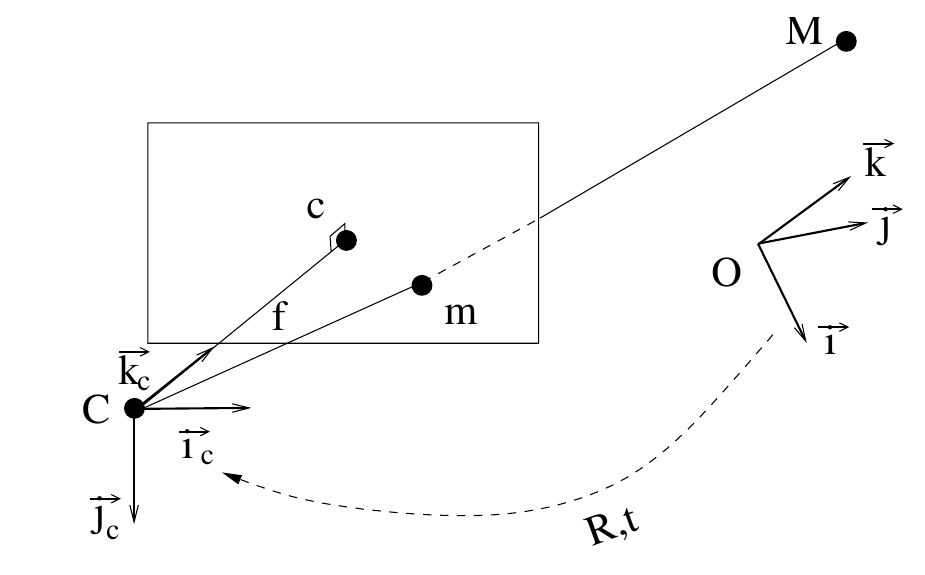
\includegraphics[width=5in]{monografia/projection_scheme.png}
\caption{Esquema de projeção em perspectiva. Observe na imagem que $(\mathbf{O}, \vec{i}, \vec{j}, \vec{k})$ é o sistema de coordenadas do mundo, $(\mathbf{C}, \vec{i_c}, \vec{j_c}, \vec{k_c})$ é o sistema de coordenadas da câmera, $\mathbf{M}$ é um ponto 3D e $\mathbf{m}$ é sua projeção 2D no plano. Imagem retirada de \cite{lepetit}.}
\label{projection_scheme}
\end{figure}

Ainda na equação \eqref{matrix_p}, $[R | t]$ é uma matriz $3 \times 4$ e representa os parâmetros extrínsecos da câmera. Diferente dos parâmetros intrínsecos, os extrínsecos mudam no decorrer do rastreamento.

Ao observar a equação \eqref{projection_eq} pode-se dizer que tendo um ponto 2D $\tilde{m}$ da imagem e um fator de escala $s$ (que também é conhecido), para que o ponto $\tilde{M}$ seja projetado em $\tilde{m}$ é necessário descobrir a matriz $P$ da câmera que realize essa operação, ou seja, um $P$ que torne $P\tilde{M_i} \equiv \tilde{m_i}$ válido para todo $i$. Como foi visto em \eqref{matrix_p}, $K$ é um parâmetro conhecido da câmera, então o que queremos descobrir, na verdade, é a matriz $[R | t]$, que a partir deste momento do texto iremos chamar de pose da câmera.

\subsection{Cálculo da pose}

O cálculo da pose é uma estimativa para que o ponto $\tilde{M_i}$, ao ser projetado em coordenadas de tela ($P\tilde{M_i}$), seja o mais próximo possível do ponto $\tilde{m_i}$, que é um ponto 2D extraído da imagem. A distância do ponto projetado $P\tilde{M_i}$ para seu correspondente extraído da imagem ($\tilde{m_i}$) é chamada de erro de reprojeção. O objetivo das técnicas de rastreamento que usam essa representação de câmera é encontrar uma pose ($[R | t]$) cuja soma dos erros de reprojeção seja a menor possível. Em outras palavras, deseja-se resolver a equação

\begin{equation}
[R | t] = \argmin_{[R | t]} \sum_i \text{dist}^2(P\tilde{M_i}, \tilde{m_i})
\label{calculo_pose}
\end{equation}

Essa equação não fornece uma solução polinomial de forma fechada, por isso métodos de otimização como o Gauss-Newton \cite{gauss_newton} ou o Levenberg–Marquardt \cite{levenberg} devem ser utilizados.

Estimadores robustos como um \emph{M-estimator} \cite{m_estimator} também podem ser utilizados, e são bastante úteis para auxiliar em uma solução adequada. O papel principal destes estimadores é eliminar a influência de \emph{outliers}, que são algumas poucas correspondências 2D-3D grosseiramente erradas, mas que podem influenciar bastante negativamente no resultado final.

\section{Rastreamento de objetos}

Para auxiliar no cálculo da pose é preciso extrair \emph{features}, que são componentes mais simples da cena como marcadores \cite{ref_marcadores}, arestas do objeto \cite{ref_arestas}, textura do objeto \cite{ref_textura}, e pontos de interesse \cite{ref_pontosdeinteresse}, que auxiliem na recuperação da pose (3D) da câmera virtual a partir de uma sequência de imagens 2D. Conhecendo a posição 3D dessas \emph{features} no quadro anterior e extraindo sua posição 2D no quadro atual já é um grande passo para realizar o rastreamento. A intenção dos algoritmos de rastreamento é descobrir uma pose da câmera que, ao usá-la para fazer a projeção 2D destas \emph{features} 3D, essas \emph{features} tenham as mesmas posições 2D das que foram extraídas do quadro atual.

Como foi dito anteriormente, existem na literatura vários tipos de informações que podem ser usadas como \emph{features}. Uma das formas mais conhecidas de rastreamento é a que insere marcadores fiduciais na cena, como o da \figref{marcador_modelo}. Nesta técnica deve-se conhecer \emph{a priori} o marcador a ser utilizado. O trabalho consiste então em encontrar o marcador em cada quadro e saber que operação feita na câmera (rotação, translação ou cisalhamento) deixaria o marcador tomado como modelo (\figref{marcador_modelo}) com a mesma configuração que o marcador extraído da imagem (\figref{marcador_extraido}).

\begin{figure}[!ht]
	\centerline{
		\subfloat[Exemplo de marcador artificial.]{
			
\includegraphics[width=0.25\textwidth]{monografia/pattSample1}
			\label{marcador_modelo}
		}
		\hfil
		\subfloat[Exemplo de marcador extraído de uma imagem.]{
			\begin{tikzpicture}
				\pgftext[at=\pgfpointorigin]{
					\pgflowlevel{\pgftransformcm{1}{0.7}{0}{1}{\pgfpoint{0}{0}}}
					% \pgfdeclareimage[height=0.2\textwidth]{deformedtag}{monografia/pattSample1} % on preample
					% \pgfuseimage{deformedtag}
					
\includegraphics[height=1in]{monografia/pattSample1}
				}
			\end{tikzpicture}
			\label{marcador_extraido}
		}
	}
	\caption{Exemplo de marcador e sua projeção.}
\end{figure}

O uso de marcadores, no entanto, requer que uma interferência no ambiente seja feita e, apesar de simplificar o rastreamento 3D, nem sempre pode ser usado. Isto acontece porque podem existir limitações técnicas que impeçam a introdução prévia de elementos auxiliares no ambiente real ou podem até existir restrições baseadas na decisão do usuário final. Neste caso deve-se buscar \emph{features} que estejam naturalmente presentes na cena, o que muitas vezes ocorre quando elas são parte do próprio objeto a ser rastreado. Abrir mão de marcadores artificiais torna o rastreamento muito mais desafiador, e a discussão dessas técnicas será o foco do resto deste trabalho de graduação.

Existem várias formas de rastrear um objeto na cena sem a utilização de marcadores externos \cite{lima2010model} e entre elas existe o rastreamento baseado em modelo e o \emph{Structure from Motion} (\emph{SfM}).

O rastreamento baseado em modelo é caracterizado pelo uso de um modelo 3D pré-definido do objeto a ser rastreado. O modelo serve para saber as características do objeto que serão usadas para rastrear. Já na técnica baseada em \emph{SfM} \cite{lima2010model} não é necessário um conhecimento prévio da cena e, por isso, é bastante útil quando o ambiente a ser rastreado é desconhecido.

Ao se comparar as duas abordagens pode-se dizer que a baseada em modelos é computacionalmente mais eficiente que a \emph{SfM} \cite{drummondecipolla}. A \emph{SfM} baseia-se na análise de todo o \emph{frame} da sequência de vídeo para poder identificar um movimento na câmera, e sabendo-se que poucos segundos de um vídeo podem conter bastante informação, essa análise pode se mostrar lenta computacionalmente. A técnica baseada em modelos, por sua vez, pode tirar proveito de um modelo já conhecido do objeto a ser rastreado. Com isso apenas características chaves precisam ser analisadas para o rastreamento. Neste trabalho de graduação a técnica baseada em modelos é explorada.

\subsection{Rastreamento sem marcadores baseado em modelo}

Algumas das técnicas de rastreamento sem marcadores, como foi dito anteriormente, baseiam-se no uso de um modelo 3D (construído em uma ferramenta CAD como o 3D Studio Max \cite{ref_3dsmax} ou Maya \cite{ref_maya}) do objeto a ser rastreado \cite{lepetit}. Ter esse modelo é importante, já que a maioria das técnicas de rastreamento sem marcadores utiliza \emph{features} do próprio objeto. Considerando uma análise superficial, a ideia é equivalente ao método que utiliza marcadores: extrair as \emph{features} da imagem 2D capturada e tentar chegar a uma pose da câmera virtual que, ao ser usada para fazer a projeção 2D do modelo 3D do objeto, chegamos a uma imagem equivalente àquela capturada do objeto.

As técnicas baseadas em modelo podem usar uma gama de informações do objeto para dar suporte ao processo de rastreamento, sendo uma delas a textura do objeto \cite{lima2010model}. O rastreamento baseado em textura pode ser feito de diferentes formas: uma das técnicas aplica um modelo de distorção a uma imagem de referência \cite{ref_19tgchico}; outra utiliza pontos de interesse, e se baseia no casamento de \emph{features} das imagens recuperadas com \emph{features} de uma imagem de template pré-definida \cite{lepetit}.

Além da textura do objeto, um outro tipo de informação que pode ser usada são as suas arestas \cite{lepetit}. O processo de casamento de aresta pode ser descrito da seguinte forma: tendo as arestas do modelo CAD pré-definido, o objetivo é encontrar os pontos de forte gradiente da imagem para formar linhas (que serão as arestas do objeto) e então encontrar a pose que projeta as arestas do modelo 3D o mais próximo possível das arestas extraídas da imagem.

A escolha entra textura ou arestas do modelo depende do objeto a ser rastreado. A \figref{textura_aresta_textura} ilustra um objeto com textura cujas arestas não são bem definidas. Se for feita uma rotação do objeto no eixo $Z$, conforme mostrado na imagem, dificilmente um algoritmo baseado em arestas irá percebê-la corretamente. Por outro lado, o objeto mostrado na \figref{textura_aresta_aresta}, apesar de não ter textura, tem arestas bem definidas. No presente trabalho as técnicas de rastreamento baseado em arestas são investigadas.

\begin{figure}[!ht]
	\centerline{
		\subfloat[Este objeto, por ser cilíndrico, não possui arestas bem definidas. No entanto seu desenho é um convite ao uso de técnicas de rastreamento baseadas em textura.]{
			\shortstack{\textbf{FAZER:} Lata de coca-cola com\\um eixo Z atravessando no meio}
			\label{textura_aresta_textura}
		}
		\hfil
		\subfloat[Este objeto não possui textura, porém suas arestas são bem definidas. Imagem retirada de \cite{marchand_modelbased}.]{
			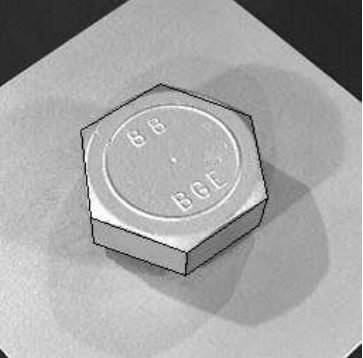
\includegraphics[width=0.25\textwidth]{monografia/textura_aresta_aresta}
			\label{textura_aresta_aresta}
		}
	}
	\caption{Dois tipos de objetos: um com textura e outro com arestas bem definidas.}
\end{figure}

\subsection{Técnicas de rastreamento baseado em arestas}

Independente das técnicas que serão apresentadas abaixo, o rastreamento baseado em arestas segue praticamente o mesmo \emph{pipeline}. Primeiro é preciso saber a pose do \emph{frame} anterior. Se for o primeiro \emph{frame} este, ainda assim, terá que ser informado, e é por isso que nos experimentos é preciso definir uma pose inicial. Depois de obtida a pose do \emph{frame} anterior, o \emph{frame} atual é capturado a partir de uma sequência de vídeo. Essa imagem capturada será então analisada em busca de pontos de forte gradiente para a extração de bordas. Obtém-se então as arestas do modelo que estão visíveis após serem projetadas utilizando a pose do quadro anterior. As arestas visíveis são aquelas que ao serem projetadas na tela não são oclusas por outras partes do objeto (considerando um objeto opaco). Em seguida, a projeção das arestas visíveis é comparada com as bordas extraídas da imagem. Nessa comparação é feito um casamento entre a aresta 3D projetada do modelo e a aresta extraída da imagem (veja \figref{cubo_pipeline_drummond}). Esse casamento dá à aresta extraída da imagem uma estimativa inicial de sua posição 3D. Após isso é feito o cálculo da pose para que as arestas do modelo 3D projetado na tela, utilizando a pose calculada, fiquem o mais próximo possível das arestas extraídas da imagem. Esta pose será então a pose do \emph{frame} atual.

\begin{figure}[!ht]
\centering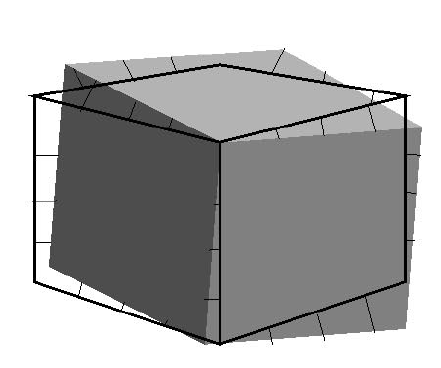
\includegraphics[width=2in]{monografia/cubo_pipeline_drummond}
\caption{Casamento de arestas do modelo (\emph{wireframe}) com arestas do objeto na imagem (cubo cinza). Imagem retirada de \cite{drummondecipolla}.}
\label{cubo_pipeline_drummond}
\end{figure}

Como descrito no \emph{pipeline}, uma das etapas do rastreamento baseado em arestas é a extração das arestas do quadro atual, que é uma imagem 2D. Duas técnicas importantes a serem mencionadas são a extração explícita de aresta \cite{extracao_explicita} e a técnica da amostragem de pontos\cite{drummondecipolla}.

\label{sec:extracao_explicita}
Na primeira técnica são extraídos segmentos de reta da imagem utilizando algum algoritmo de detecção de linha, como a transformada de Hough, ao mesmo tempo em que o modelo é renderizado utilizando a pose do \emph{frame} anterior, como mostra a \figref{carro_extracao_explicita}. Um procedimento recursivo é então utilizado com a finalidade de encontrar as melhores correspondências entre as arestas do modelo 3D e os segmentos de reta 2D extraídos da imagem. Neste procedimento as arestas projetadas do modelo são agrupadas com os segmentos de reta extraídos de acordo com a menor distância de Mahalanobis. Na sequência a técnica da amostragem de pontos é explicado, tendo sido o alvo principal de pesquisa deste trabalho de graduação.

\begin{figure}[!t]
\centering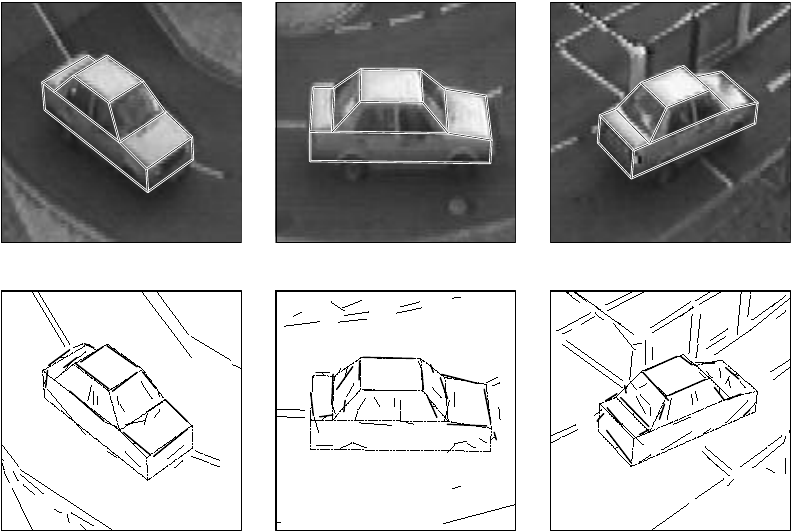
\includegraphics[width=0.9\textwidth]{monografia/carro_extracao_explicita}
\caption{Processo de extração explícita de arestas. Imagem retirada de \cite{extracao_explicita}.}
\label{carro_extracao_explicita}
\end{figure}

\subsection{Amostragem de pontos}
\label{sec:amostragem_de_pontos}

A técnica de amostragem de pontos \cite{drummondecipolla} apresenta outra maneira de fazer o casamento entre as arestas do modelo e as arestas do objeto. Neste caso as arestas da imagem não são extraídas explicitamente para depois serem comparadas com as arestas projetadas no modelo, como na abordagem anterior.

Cada aresta do modelo, que será chamada de $E_i$, é dividida de modo que se obtenha $n_i$ pontos amostrados, sendo $\{e_{i,j}\}$ o conjunto dessas amostras de $E_i$. A técnica de amostragem de pontos associa pontos do modelo 3D com pontos 2D extraídos da imagem. A extração desses pontos é feita a partir de uma busca de pontos de forte gradiente, chamados de $e'_{i,j}$, na normal de cada amostra $e_{i,j}$, como pode ser visto na \figref{amostragem_de_pontos}.

\begin{figure}[!ht]
\centering\includegraphics{monografia/sample_point_diagram}
\caption{Diagrama de pontos amostrados. Pode-se observar que a aresta $E_0$ da imagem possui $n_0$ amostras e cada uma delas está associada a uma hipótese $e'_{i,j}$, resultado da busca na normal da amostra.}
\label{amostragem_de_pontos}
\end{figure}

Tendo em vista esse casamento de amostras do modelo com amostras do objeto, o objetivo do algoritmo é encontrar uma pose que minimize a diferença entre a projeção da amostra, $P \cdot e_{i,j}$, e seu correspondente na imagem capturada. Utilizando a equação \eqref{calculo_pose}, o problema pode ser descrito como

\begin{equation}
[R | t] = \argmin_{[R | t]} \sum_i \text{dist}^2(P \cdot e_{i,j}, e'_{i,j})
\label{calculo_pose_amostragem}
\end{equation}

É importante lembrar que somente as arestas visíveis do modelo são usadas, porém pode existir o caso em que a aresta esteja parcialmente visível, e uma das vantagens desta abordagem é poder lidar com esse caso, como mostra a \figref{occlusion}.

Outra vantagem é que a busca por pontos de forte gradiente na imagem é bastante simplificada. Ela acontece apenas em uma dimensão e somente nas normais das amostra do modelo o que torna a execução do algoritmo bastante rápida.

\subsection{Múltiplas hipóteses}

Um dos problemas que ocorrem nas técnicas baseadas em arestas é que nem sempre se consegue extrair com precisão as arestas da imagem. Na busca por pontos na normal da amostra pode existir mais de um ponto de forte gradiente devido ao ruído da câmera, objetos externos na cena, sombra do objeto ou até arestas do próprio objeto, dependendo da pose. A \figref{cubo_0} ilustra um exemplo em que mais de um ponto de forte gradiente é encontrado.

\begin{figure}[ht!]
\centering
\includegraphics{monografia/cubo_exemplo}
\caption{O cubo azul representa o modelo da pose anterior; a imagem do cubo é a cena atual da qual pretende-se extrair a pose; os pontos vermelhos são as amostras do modelo; e os pontos em formato de X são as correspondências encontradas na cena atual. Nota-se que devido a ruídos na imagem algumas amostras possuem mais de uma correspondente.}
\label{cubo_0}
\end{figure}

Neste caso é preciso escolher com qual dos pontos achados será feito o casamento da amostra. Uma das alternativas para a escolha do ponto extraído seria escolher a opção de maior gradiente. No entanto essa escolha nem sempre é uma boa opção, pois um alto contraste nem sempre significa que o ponto tem maiores chances de pertencer ao modelo. Na \figref{sem_multiplas_hipoteses} observa-se que objetos externos podem confundir o casamento das amostras.

\begin{figure}[!ht]
	\centerline{
		\subfloat[Experimento com hipótese única. Observe que os pontos do controle remoto (de maior contraste) confundem o rastreamento.]{
			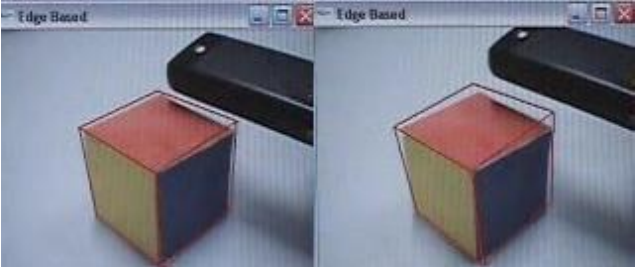
\includegraphics[width=0.5\textwidth]{monografia/sem_multiplas_hipoteses}
			\label{sem_multiplas_hipoteses}
		}
		\hfil
		\subfloat[Experimento com múltiplas hipóteses.]{
			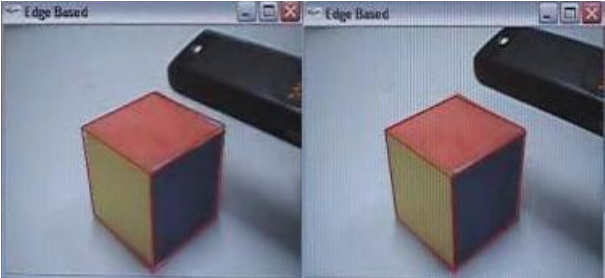
\includegraphics[width=0.5\textwidth]{monografia/com_multiplas_hipoteses}
			\label{com_multiplas_hipoteses}
		}
	}
	\caption{Resultado de um rastreamento com múltiplas hipóteses e com hipótese única.}
\end{figure}

Para este tipo de problema uma boa solução é o uso de múltiplas hipóteses da amostra \cite{multiplas_hipoteses}. Ou seja, cada amostra $e_{i,j}$ está associada a um conjunto de hipóteses $\{e'_{i,j,l}\}$, e somente as correspondências mais prováveis seriam usadas no processo de minimização. Na prática essa técnica é menos vulnerável a mudanças no ambiente. Na \figref{com_multiplas_hipoteses} é mostrado o resultado de uma técnica de rastreamento com múltiplas hipóteses de amostra. Observe que mesmo aproximando um objeto com forte gradiente, o rastreamento sofre pouca distorção.

Para fins práticos as hipóteses mais prováveis são aquelas que mais se aproximam da amostra projetada. Utilizando estas informações e a equação \eqref{calculo_pose_amostragem} pode-se chegar à seguinte fórmula de cálculo de pose:

\begin{equation}
[R | t] = \argmin_{[R | t]} \sum_i \text{dist}^2(P \cdot e_{i,j}, \text{mindist}(e'_{i,j,l}, P \cdot e_{i,j}))
\end{equation}

\noindent
em que $\text{mindist}(e'_{i,j,l}, P \cdot e_{i,j})$ resulta na hipótese com a menor distância da amostra projetada.

\begin{comment}
\section{NULL! Seção a ser reescrita}

Pule para o próximo capítulo
% Uma outra técnica de rastreamento é a baseada em \emph{Structure from Motion} (\emph{SfM}) \cite{teichrieb2007survey}. Nesta abordagem não é necessário um conhecimento prévio da cena e, por isso, é bastante útil quando o ambiente a ser rastreado é desconhecido. Apesar disso, a \emph{SfM} tem a desvantagem de ser bastante complexa e não tão eficiente para rastrear uma sequência em vídeo. Isso se deve ao fato de um vídeo conter bastante informação, e muitas vezes apenas uma pequena parte disso seria suficiente para rastrear o movimento da câmera \cite{drummondecipolla}. É nesse aspecto que o rastreamento baseado em modelos se destaca, pois são observados apenas pontos chaves da cena (como os contornos do modelo, por exemplo).

\section{Rastreamento por arestas}

%Para a extração das arestas da imagem geralmente são utilizados algoritmos de detecção de borda, como o filtro Sobel.

% A vantagem dessa técnica é que arestas são relativamente mais fáceis de serem encontradas em uma imagem. Algoritmos para detecção de bordas são abundantes na literatura e já vem sido bastante estudado em processamento de imagens.%citation

\subsection{Técnicas}

Uma das formas de fazer o casamento entre as arestas do modelo e as arestas da imagem é usar o que pode ser chamado de extração explícita das arestas. Utilizando algum algoritmo de detecção de linha, como a transformada de Hough, as arestas da imagem são extraídas para depois serem comparadas com as do modelo na pose anterior. %cite (Hough) [3] em VTetal

% [como funciona?]. Entretanto um dos problemas desse método é a possibilidade de parte de uma aresta visível estar oculta [como mostra a figura, retirada de \cite{drummondecipolla}]. Isso pode ser interpretado pelo algoritmo como duas arestas menores e que possivelmente não vai ser casada com a aresta correspondente do modelo.

Outra forma de trabalhar com rastreamento baseado em arestas é utilizando a técnica de amostragem de pontos. Neste caso a aresta do modelo é dividida em partes iguais, chamados de amostras (ou \emph{sample-points}). Cada ponto amostrado é então comparado com pontos de forte gradiente da imagem que estão próximos da aresta. Uma das formas de fazer isso é fazer uma busca na direção normal da aresta que passa pelo ponto amostrado. O primeiro ponto de forte gradiente encontrado pode então ser considerado correspondente ao ponto amostrado. Ou seja, é possivelmente onde aquele ponto da pose anterior está no \emph{frame} atual.

% que serão utilizados para casar com as amostras extraídas da imagem.

Em outras palavras o casamento das amostras do modelo com os pontos extraídos da imagem acontece da seguinte forma: primeiro o modelo do \emph{frame} anterior é renderizado a fim de ter uma estimativa inicial da posição do objeto no frame atual; Para cada aresta do modelo são extraídos $N$ amostras que posteriormente serão comparadas com a imagem obtida do frame atual; Em cada amostra do modelo é feita uma busca na normal da aresta a fim de encontrar pontos de forte gradiente (bordas), o que podemos supor que são pontos da aresta da imagem. A partir do casamento das amostras do modelo com os pontos de forte gradientes da imagem, pode ser feita uma estimativa do movimento da câmera.

A extração explícita das arestas tem a vantagem de ser mais robusta, porém é restrita apenas a objetos poligonais. A amostragem de pontos, por sua vez, mostra-se bastante útil quando as arestas não são formadas por retas. Há também a vantagem de trabalhar melhor com arestas oclusas, como mostra a \figref{occlusion}.
\end{comment}

\begin{figure}[ht!]
\centering
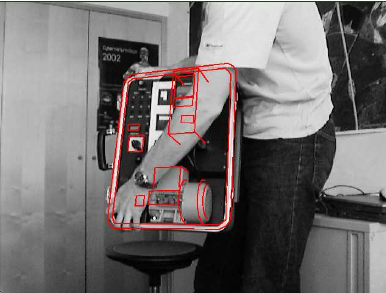
\includegraphics{monografia/occlusion.png}
\caption{Objeto com oclusão parcial das arestas. Imagem retirada de \cite{wuest}.}
\label{occlusion}
\end{figure}

% Na primeira técnica a aresta parcialmente oclusa seria considerada duas arestas diferentes, enquanto que a amostragem de pontos seria capar de identificá-la como uma aresta só.

\begin{comment}
\subsection{Trabalhando com múltiplas hipóteses}

Algo comum de acontecer na etapa de casamento das amostras do modelo com os pontos de forte gradiente da imagem é que, ao percorrer a normal para achar pontos de forte gradiente, a busca pode retornar mais de um resultado. Ou seja, é possível haver mais de uma hipótese de pontos da imagem para serem casados com uma amostra do modelo. [isso parece ser muito específico]

\subsection{Rascunho}

extração explícita de arestas (ruim por causa da oclusão \cite{drummondecipolla}) \\
amostragem de pontos (sample points. a que eu uso) \\

renderizar o modelo, localizar as arestas visiveis do modelo. a partir dela, extrair sample points. tentar fazer um match das arestas do modelo com as arestas da imagem obtida\cite{drummondecipolla} \\
explicar que pegamos uma aresta do modelo, pegamos alguns sample points. a partir dos sample points seguimos pela normal do ponto e tentamos achar os pontos de forte gradiente. podem existir vários pontos de forte gradiente para um único \emph{sample point} (múltiplas hipóteses) \\

explicar como a escolhas das múltiplas hipóteses podem ser feitas. deixar um gancho para o capítulo seguinte que explica como fazer a escolha utilizando o k-means \\

outliers happens. podem ter outras coisas que formam uma aresta. \\
\end{comment}

\begin{comment}
Em um reprodução de vídeo, rastrear um objeto se caracteriza por identificar a sua posição na cena quando tanto o objeto quanto a câmera está em movimento \cite{lepetit}.

Um vídeo contém bastante informação e é preciso extrair apenas parte dela. Por isso que é usada uma técnica \emph{feature-based}, em que o processamento das imagens é restrito à localização de pontos de forte gradiente como os contornos do objeto \cite{drummondecipolla}.

Uma das formas de efetuar um rastreamento é utilizando um técnica baseada em modelos. Nesse tipo de técnina é necessário um conhecimento prévio do que vai ser rastreado. No caso, é preciso já ter um modelo 3D do objeto a ser rastreado.

* Tipos de rastreamento: SfM, Model based

sfm pega a cena toda.
model based precisa de um modelo 3D pré-construído
    * edge based
        * amostragem de pontos (sample points. é o que eu uso)
        * extração explícita das arestas (ruim por causa da oclusão \cite{drummondecipolla})
    * texture based


model based é mais simples que sfm, mas é preciso ter um modelo de antemão \cite{teichrieb2007survey}

renderizar o modelo, localizar as arestas visiveis do modelo. a partir dela, extrair sample points. tentar fazer um match das arestas do modelo com as arestas da imagem obtida\cite{drummondecipolla}

outliers happens. podem ter outras coisas que formam uma aresta. esse é o problema que eu quero resolver.

Uma das etapas mais importantes de aplicações com realidade aumentada é o rastreamento e registro da cena \cite{teichrieb2007survey}.

Falar sobre o que é rastreamento. Etapas do rastreamento: pegar imagens da camera, identificar?
\end{comment}
